\documentclass[11pt]{article}
\usepackage[T1]{fontenc}
\usepackage{lmodern}
\usepackage[margin=1in]{geometry}
\usepackage{amsmath,amssymb,amsthm,mathtools}
\usepackage{booktabs,longtable,tabularx,array}
\usepackage{enumitem,graphicx,xcolor,microtype,hyperref}
\usepackage[nameinlink,noabbrev]{cleveref}
\usepackage[numbers,sort&compress]{natbib}
\usepackage{tikz}
\usetikzlibrary{arrows.meta,positioning,calc,fit,decorations.pathreplacing}
\hypersetup{colorlinks=true,linkcolor=blue!55!black,citecolor=blue!55!black,urlcolor=blue!55!black,
pdftitle={Raw Strongly Tree-Child Level-2 Species Networks from Metric Genealogy Laws under the NMSC},
pdfauthor={Alec Kriebel}}
\setlist[itemize]{leftmargin=1.5em,itemsep=2pt,topsep=4pt}
\setlist[enumerate]{leftmargin=1.7em,itemsep=2pt,topsep=4pt}
\newtheorem{theorem}{Theorem}[section]
\newtheorem{lemma}[theorem]{Lemma}
\newtheorem{proposition}[theorem]{Proposition}
\newtheorem{corollary}[theorem]{Corollary}
\newtheorem{definition}[theorem]{Definition}
\newtheorem{remark}[theorem]{Remark}
\newtheorem{example}[theorem]{Example}
\newtheorem{assumption}[theorem]{Assumption}
\newcommand{\CCR}{\operatorname{CCR}}
\newcommand{\Qraw}{\mathcal Q^{\mathrm{NMSC,raw}}_2}
\newcommand{\Qdirect}{Q^{\mathrm{direct}}_2}
\newcommand{\Rraw}{\mathfrak R}
\newcommand{\tr}{\operatorname{tr}}
\newcommand{\rank}{\operatorname{rank}}
\newcommand{\diag}{\operatorname{diag}}
\newcommand{\supp}{\operatorname{supp}}
\newcommand{\dd}{\,\mathrm d}
\newcommand{\one}{\mathbf 1}
\newcommand{\R}{\mathbb R}
\newcommand{\Ncal}{\mathfrak N}
\newcommand{\GT}{\operatorname{GT}}
\newcommand{\Law}{\operatorname{Law}}
\newcommand{\Part}{\operatorname{Part}}

\title{\textbf{Raw Strongly Tree-Child Level-2 Species Networks from Metric Genealogy Laws under the NMSC}\\[3pt]
Signed pair co-occupancy, rooted graph reconstruction, and demographic fibers}
\author{Alec Kriebel\\Independent Researcher\\\small\href{https://orcid.org/0009-0001-9320-500X}{ORCID: 0009-0001-9320-500X}\quad DOI: \href{https://doi.org/10.5281/zenodo.22729545}{10.5281/zenodo.22729545}}
\date{September 5, 2026}

\begin{document}
\maketitle

\begin{abstract}
We classify the observable rooted graph and parameters of finite strict temporally separated binary strongly tree-child species networks of level at most two under the independent-lineage Network Multispecies Coalescent (NMSC), with a fixed known surjective taxon sampling map. Equality of complete normalized rooted metric-genealogy laws is equivalent, pointwise on the full positive domain, to an explicit quotient generated by eight move types.

The proof recovers current pair co-occupancy from the analytic germ of a finite positive Kingman mixture. Signed jumps reveal every tree event and every pair-exposed reticulation. Descendant clusters, chronology, tree-childness and level-two shortcut completion then reconstruct the retained graph, including arbitrary decorations. Deterministic witnesses and actual three-lineage merger densities recover oriented inheritance weights and the entire finite demographic rate words on exposed populations. Scalar propagation through ancestral reticulations links both incoming arms, including equal rates and inheritance one-half. The indexed collection of all genealogy marginals on at most three sampled lineages suffices for the complete quotient.

A reticulation with one descendant sampled lineage retains its two typed first-exposure outlets and route weights, while its internal clock and singly occupied demographic words are unobservable. Sister-transfer direction is invisible exactly when both sides are sample unary; the corresponding reversal transfers the whole exposed donor rate word. Together with presentation suppression, equal-rate composition, unary-corridor replacement, parent exchange and labelled isomorphism, these responses exhaust the quotient. Exact hidden-clock and rank-one nonbridge examples explain essential obstructions. A separate graph argument derives the five cores and twelve minimum strong repairs.

The companion study transfers the classification to all indexed ordered locus laws with known boundaries, jointly with the stationary distribution and trace-normalized shared irreducible stationary reversible substitution generator. The reconstruction uses observable current-grouping scalars throughout.
\end{abstract}

\section{Introduction}
The observation in this paper is the complete probability law of rooted metric gene genealogies generated by an NMSC presentation.  Population occupancy and reticulation-route labels are latent.  The companion study \citep{KriebelNMSCCore2026} proves, on its strict stationary reversible domain,
\begin{equation}
 (\mathbb P^{(L)}_\xi)_{L\ge1}
 \Longleftrightarrow
 (\pi,Q_0,\bar\mu_{\rm metricGT})
 \Longleftrightarrow
 (\pi,Q_0,\CCR),
 \qquad Q_0=Q/(-\tr Q).
 \label{eq:bridge}
\end{equation}
The present paper starts from $\bar\mu_{\rm metricGT}$ and identifies the positive rooted population-network quotient that generated it.

Prior NMSC work already shows that distinguishability depends on allele sampling and is not determined by displayed-tree sets, including examples of metric-genealogy ambiguity \citep{ZhuDegnan2017}.  At coarser observations, quartet gene-tree probabilities recover the tree of blobs and substantial level-1 structure \citep{AllmanBanosMitchellRhodes2023,AllmanBanosGarroteRhodes2024}, and higher-level identifiability is known for a class of galled tree-child networks \citep{AllmanAneBanosRhodes2025}.  For semi-directed outer-labelled planar galled level-2 networks, \citet{HoltgrefeEtAl2025} characterize a canonical form from displayed quartets, with NMSC applications; we refer to the corrected version \citep{HoltgrefeEtAl2026Correction}.  Those observation maps and graph classes differ from the complete rooted metric-genealogy law and graph-and-parameter quotient considered here.

The main inverse uses two distinct kinds of information.  First, signed
jumps of a scalar current co-occupancy probability recover a global labelled
ancestry order.  Completing its cover edges under binary tree-child and
level-two constraints gives the retained rooted graph.  Second, positive
local merger densities recover parameters on those already identified
incidences.  A unary reticulation remains a typed two-outlet response because
one lineage cannot record a coalescent clock before meeting another lineage.

All statements compare two supplied positive NMSC realizations.  No minimal
linear realization of the observed behavior is interpreted as a biological
network.  In particular, we do not extract historical route-conditioned
future laws: after two routes reconverge those laws can coincide, so a
projector that distinguishes the routes need not descend to the observable
quotient.  The current grouping scalar used here follows instead from a
finite positive frozen-epoch germ.

\subsection{Main results}
Let $X$ be the taxon set, $S$ the sampled-lineage set, and $\mathfrak s:S\to X$ the known sampling map.  Let $\Ncal_{\mathrm{STC},2}(X,S,\mathfrak s)$ be the raw class in \cref{sec:model}.  Its members are strict, temporally separated, rooted binary temporal strongly tree-child NMSC presentations of level at most two with independent lineage routing.

The main theorem is the following pointwise classification.

\begin{theorem}[Raw level-2 metric-genealogy classification]
\label{thm:main}
For any
\[
 (N,\eta),(N',\eta')\in\Ncal_{\mathrm{STC},2}(X,S,\mathfrak s),
\]
\begin{equation}
 \bar\mu^{\rm metricGT}_{N,\eta}=\bar\mu^{\rm metricGT}_{N',\eta'}
 \quad\Longleftrightarrow\quad
 \Qraw(N,\eta;\mathfrak s)=\Qraw(N',\eta';\mathfrak s).
 \label{eq:headline}
\end{equation}
The quotient is generated by eight explicit move types:
\begin{enumerate}[label=\textup{(Q\arabic*)}]
\item suppression of parameter-free degree-two vertices;
\item composition of co-located presentational factors of the same fixed boundary operator, without introducing another biological event;
\item merger of adjacent equal-rate demographic epochs on one unchanged population lineage;
\item contraction or contextual replacement of maximal sample-unary corridors;
\item parent-presentation exchange with $\gamma\leftrightarrow1-\gamma$;
\item bi-unary sister-triangle reversal with the exact exposed donor-rate-word transfer;
\item labelled graph isomorphism preserving all retained normalized times, exposed rates, retained routing parameters, sampled-lineage assignments, and port words;
\item replacement of a maximal pre-exposure unary routing fan by another positive fan with the same normalized singleton input and the same unordered pair of typed first-exposure outlet weights; its internal event time and singly occupied demographic words are not retained.
\end{enumerate}
No further graph or parameter move occurs on the stated strict, temporally separated class.  In particular, no externally cited simultaneous-BDI action is used as a generator of this principal quotient.
\end{theorem}

\begin{corollary}[Direct-sequence classification]
\label{cor:sequence}
Under the assumptions of the companion study \citep{KriebelNMSCCore2026}, two level-at-most-two presentations in the class above have identical indexed direct locus laws if and only if
\[
 \pi=\pi',\qquad Q_0=Q'_0,
 \qquad
 \Qraw(N,\bar\eta;\mathfrak s)=\Qraw(N',\bar\eta';\mathfrak s).
\]
Here $\bar\tau=(-\tr Q)\tau$ and $\bar\lambda=\lambda/(-\tr Q)$.  The graph conclusion is therefore uniform over all irreducible stationary reversible finite-state substitution generators covered by the companion study.
\end{corollary}

The local direction theorem is exact.

\begin{theorem}[Sister-triangle exposure theorem]
\label{thm:triangle}
A strict sister-transfer direction is invisible in the complete metric-genealogy law if and only if both sister ports are sample unary, modulo pre-exposure unary-fan replacement and the bi-unary donor-rate-word move.  If either side is pair exposed, the direction is pointwise identifiable modulo parent presentation.
\end{theorem}

\begin{corollary}[One lineage per taxon]
\label{cor:one-sample}
If $|\mathfrak s^{-1}(x)|=1$ for every $x\in X$, a sister triangle is direction-ambiguous exactly when both side clusters contain one taxon.  Every nonsister direction and every sister direction with a nonsingleton side cluster is retained by $\Qraw$.
\end{corollary}

\begin{corollary}[Exposure-complete sampling]
\label{cor:exposure}
If every sister-triangle side is pair exposed, every ordinary triangle is oriented.  The sufficient condition $|\mathfrak s^{-1}(x)|\ge2$ for every terminal taxon is stronger than necessary but guarantees exposure completeness.
\end{corollary}


\begin{figure}[ht]
\centering
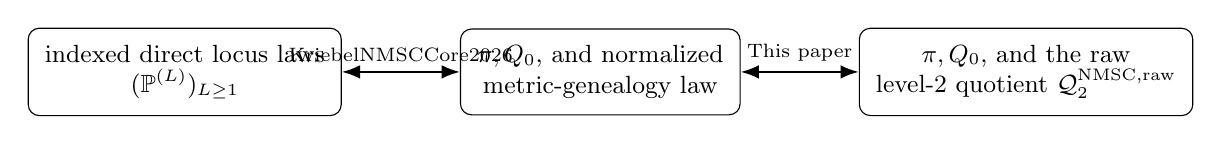
\begin{tikzpicture}[>=Latex,node distance=1.2cm and 1.5cm,every node/.style={font=\small}]
\node[draw,rounded corners,align=center,inner sep=6pt] (seq) {indexed direct locus laws\\$(\mathbb P^{(L)})_{L\ge1}$};
\node[draw,rounded corners,align=center,inner sep=6pt,right=of seq] (gt) {$\pi,Q_0$, and normalized\\metric-genealogy law};
\node[draw,rounded corners,align=center,inner sep=6pt,right=of gt] (qr) {$\pi,Q_0$, and the raw\\level-2 quotient $\Qraw$};
\draw[<->,thick] (seq)--node[above,font=\scriptsize]{\citep{KriebelNMSCCore2026}}(gt);
\draw[<->,thick] (gt)--node[above,font=\scriptsize]{This paper}(qr);
\end{tikzpicture}
\par\smallskip
\begin{minipage}{.92\linewidth}\scriptsize
The companion study \citep{KriebelNMSCCore2026} assumes a stationary reversible shared CTMC and known locus boundaries.
This paper assumes a strict temporal rooted strongly tree-child presentation of
level at most two.
\end{minipage}
\caption{The two-paper theorem architecture.  No displayed-tree or direct-substitution invariant is transferred across the first arrow.}
\label{fig:scope}
\end{figure}

\subsection{Why arbitrary multilineage routing does not obstruct the theorem}
If $m$ blocks reach one reticulation, the hidden routing boundary is indeed
\[
 R=\sum_{A\subseteq[m]}\gamma^{|A|}(1-\gamma)^{m-|A|}F_A.
\]
Restriction to any selected lineage subset is again an NMSC with the same $\gamma$ by sampling consistency. The complete indexed family of all pair and triple marginals first identifies one common global graph and then all its retained parameters. Thus at most three sampled lineages per query suffice even with arbitrary decorations, as proved in \cref{cor:three-suffice}; there is no need to invert the displayed $2^m$-component mixture.

\section{Model, sampling, and raw normalization}
\label{sec:model}

\subsection{Taxa and sampled lineages}
Let $X$ be a finite labelled taxon set.  Let $S$ be a finite labelled set of sampled gene lineages and
\[
 \mathfrak s:S\longrightarrow X
\]
a known surjection.  For $x\in X$, write $m_x=|\mathfrak s^{-1}(x)|\ge1$.  The species network has one terminal population indexed by each taxon $x$.  At time zero the NMSC starts with the $m_x$ distinct labelled blocks in that terminal population.  Gene-genealogy leaves are indexed by $S$, not by duplicated taxon vertices.

\subsection{Raw population networks}
A raw presentation $N$ is a finite rooted binary directed acyclic graph.  The root has indegree zero and outdegree two; a tree vertex has indegree one and outdegree two; a reticulation has indegree two and outdegree one; and terminal population leaves are indexed by $X$.  Reticulation parents are distinct in the raw biological presentation.  Parallel parent arcs and directed two-cycles are excluded there.  Parallel topological segments may appear only after unported degree-two vertices are suppressed in a generator core; every full strong repair separates the corresponding raw parents.  Vertices carry temporal coordinates increasing backward in time, and every population interval has positive duration.

Every population interval has a positive finite Kingman pair rate, constant between successive demographic or biological vertices. Each population therefore has a finite piecewise-constant rate word. A demographic rate-change vertex is permitted on an otherwise unchanged population lineage. Every reticulation has inheritance probability $\gamma\in(0,1)$, and each extant lineage block routes independently. Distinct internal biological events (tree joins and reticulations, including the root join) have distinct absolute ages in the principal theorem. All terminal samples occur at time zero. Q2 concerns only presentational factorizations of one fixed event operator; it does not admit simultaneous distinct biological events.

Above the root, all surviving blocks enter one ancestral population that continues indefinitely backward in time.  It has a finite demographic rate word followed by a constant positive pair rate.  Thus all sampled blocks ultimately coalesce almost surely, and the metric-genealogy law is a probability law on complete rooted genealogies.  The finite-duration requirement applies to finite intervals between presentation boundaries; the final ancestral epoch is unbounded.

The adjective \emph{strongly tree-child} is used in the same precise sense as in the companion level-2 topology trilogy.  Form the standard semi-directed reduction of the rooted presentation by suppressing the root in the usual way, forgetting the directions of ordinary tree edges, and retaining every reticulation arrowhead.  The presentation is strongly tree-child when this mixed topology is tree-child under every admissible rooting.  In the present binary standard setting this is equivalent to the local condition that every tail of a retained reticulation arrow has two incident ordinary edges.  In particular the supplied temporal rooting is tree-child: every internal tree vertex has a tree-vertex or terminal-population child, and every reticulation has a tree-vertex or terminal-population child.  This is strictly stronger than merely requiring the supplied rooting to be tree-child and is the condition for which the five-core/twelve-repair theorem below is valid.  The level is at most two: each undirected blob contains at most two reticulations.

\begin{definition}[Reachable block exposure]
For a population interval or subnetwork $F$, let $\epsilon(F)$ be the largest number of distinct sampled blocks that can simultaneously occupy one population of $F$ in a no-merger hidden history having positive routing probability.  This is a combinatorial reachability quantity on the strict domain.
\end{definition}

\begin{definition}[Sample-unary corridor]
A connected temporal subnetwork $F$ is a sample-unary corridor if it has one lower and one upper population boundary, has no sampled side entry in its interior, and $\epsilon(e)\le1$ on every internal population interval.  It is maximal if it is maximal under inclusion.
\end{definition}

\begin{definition}[Pre-exposure unary routing fan]
\label{def:unary-fan}
For a sampled label $s$ and population interval $e$, let
\[
 \epsilon_s(e)=\max_H\{\text{number of sampled blocks occupying }e:
             \text{the block containing }s\text{ occupies }e\},
\]
where $H$ ranges over positive no-merger hidden histories.  A
pre-exposure unary routing fan $F$ is a connected temporal subpresentation
with one typed lower population boundary $b_-$ and a finite nonempty set of
typed upper population boundaries $U_F$.  Exactly one sampled-lineage label can
enter $F$ in any positive hidden history, no other sampled block enters its
interior, every internal interval has $\epsilon_s(e)=1$, and every path from
$b_-$ to the exterior first exits at one member of $U_F$.  Each route is cut
at the first sampled side entry, first
possible two-block co-occupancy, or reconvergence with another fan path.  The
fan is maximal under extension without crossing one of those exposures.  Its
route-wise frontier need not be a temporal antichain: different routes may
first exit at different times.

Because no selected merger can occur in $F$, its first-hit behavior is the
finite stochastic vector
\[
 k_F(u)=\Pr\{s\text{ first exits }F\text{ through }u\},
 \qquad u\in U_F,\qquad \sum_{u\in U_F}k_F(u)=1.
\]
The strong-fan stopping theorem below proves that, on the stated strong
level-at-most-two class, every nontrivial such fan contains exactly one hidden
routing boundary, has exactly two scalar-separated typed outlets
$U_F=\{u_0,u_1\}$, and has response
$k_F=(\gamma,1-\gamma)$ modulo parent presentation.  Its canonical datum is
therefore the normalized lower singleton interface, the unordered typed
outlet--weight pairs
\[
 \mathsf U_F=\{(u_0,\gamma),(u_1,1-\gamma)\},
\]
and no hidden continuation basis.  The internal routing time and every rate or
demographic word on a singly occupied interval are absent.  A one-outlet
region is instead the sample-unary corridor of Q4.
\end{definition}

A Q8 fan is retained as the typed two-outlet macro
$\mathsf U(b_-,\mathsf U_F)$.  The structural and numerical inverses identify
its incidences and weights; its hidden clock is not part of that response.

\subsection{Deterministic normalization}
\begin{definition}[Raw normalization and raw quotient]
\label{def:normalization}
The raw quotient is the equivalence relation generated by the moves (Q1)--(Q8) in \cref{thm:main}.  For proof and computation we choose one deterministic normalization $\Rraw$.  It applies:
\begin{enumerate}
\item composition of presentational factors of one fixed boundary operator (Q2), a vacuous step on an unrefined biological presentation;
\item suppression of parameter-free degree-two vertices;
\item merger of adjacent equal-rate demographic epochs on an unchanged population lineage;
\item repeated contraction of sample-unary corridors to macro-arcs with the same endpoint times, choosing at each step the first inclusion-maximal corridor in the canonical labelled graph code;
\item canonical Q6 orientation of every bi-unary sister module: the side
carrying the least sampled-lineage label is chosen as recipient, and the
entire exposed donor rate word is transferred when reversal is required; if
the reversal changes which raw hidden fan realizes the response, record the
canonical compound Q6--Q8 response macro directly;
\item route-wise maximal extension of pre-exposure unary fans, followed by replacement of the first fan in canonical code order by $\mathsf U(b_-,\mathsf U_F)$;
\item a second suppression/equal-rate/corridor/Q6/fan pass, repeated until stable;
\item lexicographic parent normalization, complementing $\gamma$ when the parent order is exchanged.
\end{enumerate}
Every biological realization in an equivalence chain belongs to the stated temporally separated class. Q2 and its inverse change only the written factorization of an already fixed event operator; they neither insert an additional branching or routing event nor merge two biological ages. Thus no chain passes through an unstated larger simultaneous-event model class. Any extension to such a class would require a separate theorem.
\end{definition}

\begin{theorem}[Normalization theorem]
\label{thm:normalization}
The fixed procedure $\Rraw$ terminates, is idempotent, preserves the complete metric-genealogy law, and does not increase blob level.  Every raw presentation and its output represent the same $\Qraw$ class.
\end{theorem}

\begin{proof}
The canonical graph code makes every choice deterministic.  On a nonempty
sample-unary sister side positivity implies that exactly one sampled-lineage
label reaches the side port, so the Q6 orientation rule is unambiguous.  Order
the termination statistic first by the numbers of superfluous presentational
boundaries, raw graph vertices, and uncollapsed unary modules, and only then by
the ordered multiset of noncanonical Q6 and parent-presentation bits.  A
Q1/Q3/Q4/Q8 or boundary-composition step strictly lowers one of the count
coordinates.  A Q6 or parent-normalization step preserves all counts and
strictly lowers the final finite orientation coordinate.  Thus the process
terminates; rerunning the stable ordered passes proves idempotence.  Equal-rate
merging is ordinary semigroup composition on one unchanged population.  Inside
a sample-unary corridor no sampled pair can merge, every route has the same two
boundary times, and the routing probabilities sum to one.

For a unary fan, cut any observed marked genealogy at its route-wise first-hit
frontier.  For a lower prefix of density $a(p)$ and future cell $z$, the fan
contributes
\[
 H(p,z)=a(p)\{\gamma c_{u_0}(z)+(1-\gamma)c_{u_1}(z)\}.
\]
There is no internal selected merger density and no Kingman factor because
$\binom12=0$.  Equality of the two typed outlet weights therefore preserves
every contextual scalar cell.  Exposure is upward hereditary in the reachable
sense: once a second block can co-occupy a population with the focal block,
positivity lets both blocks survive and choose the same outcome at every later
routing boundary, so every reachable ancestral continuation has
$\epsilon_s\ge2$.  Hence the pre-exposure region is a unique initial route
cone; its one-outlet case is Q4 and its routed case is Q8.  The graph-only \cref{lem:strong-fan} proves that a
nontrivial fan has one hidden routing boundary and that distinct fan interiors
are disjoint.  On each route its first-exposure stopping boundary is unique;
the canonical labelled code resolves disjoint choices, so the stable output is
independent of the order of Q4 corridor contractions.  The canonical macro
need not be biologically realized.  In particular a size-two reciprocal law
orbit is represented by its least-label compound Q6--Q8 macro when the Q6
reversal would select a different hidden fan realization.  The macro does not
select a hidden time.  In the bi-unary case either focal has a strict raw
representative: place its unary reticulation anywhere below the earlier
parent, retain the same parent times, and transfer the entire exposed donor
word as in \cref{lem:biunary}.  The Q6 pass preserves the complete contextual
kernel by \cref{lem:biunary}, including the whole finite donor word.  Parent
normalization merely renames Bernoulli outcomes.  Suppression and both macro
replacements cannot create an undirected cycle, hence cannot increase level.
Each operation is one declared quotient move.
\end{proof}

\begin{proposition}[Retained demographic boundary dichotomy]
\label{prop:boundary}
The numerical inverse of \cref{thm:numerical-inverse} identifies each unequal
rate change on an exposed population.  Equal adjacent values merge by Q3.
A population with at most one reachable sampled block has no observable
demographic word.
\end{proposition}

\section{Observed cells, sampling consistency, and current co-occupancy}
\label{sec:bridge}
\label{sec:routing}

An observed marked cell specifies an ordered list of labelled mergers, open
intervals for their times, and no-other-selected-merger conditions.  It never
specifies population occupancy or a reticulation route.  Every such cell has a
finite sum of nonnegative hidden-history densities.  Strict positive rates,
durations, and routing weights imply that its density is positive exactly
when at least one compatible hidden history exists.

\begin{lemma}[Positive support]
\label{lem:positive-support}
Every feasible finite no-merger routing history has positive probability, and
every feasible marked merger history has positive density on its open time
simplex.
\end{lemma}
\begin{proof}
A hidden-history density is a product of positive routing weights, merger
rates, and exponential no-merger factors.  Infeasible histories contribute
zero.  The finite sum cannot cancel.
\end{proof}

\begin{theorem}[NMSC sampling consistency]
\label{thm:sampling-consistency}
Restricting a metric genealogy to any selected subset $T\subseteq S$ and
suppressing degree-two genealogy vertices gives the NMSC law on the same
population network started with just those labels.
\end{theorem}
\begin{proof}
The Kingman pair-clock construction restricts consistently to blocks meeting
$T$.  A merger with a deleted block changes neither the retained partition
nor its population.  At a reticulation the retained blocks retain independent
Bernoulli routes with the same parameter; summing deleted routes gives one.
Deterministic transport commutes with restriction.  Apply these facts along
the finite event list and the final ancestral epoch.
\end{proof}

\begin{corollary}[Subset routing identity]
\label{cor:subset-routing}
If $m$ blocks reach a reticulation, restriction to $r$ selected blocks gives
the $2^r$ assignment weights
$\gamma^{|A|}(1-\gamma)^{r-|A|}$, independently of $m$.
\end{corollary}

\begin{definition}[Pair exposure]
A population is pair exposed when two distinct sampled labels can reach it
as unmerged blocks in a positive no-merger history.  A sister side is sample
unary when exactly one sampled label can reach it.
\end{definition}

For distinct labels $i,j$, let $T_{ij}$ be their merger time in their pair
restriction, and write $f_{ij}$ for its density.  We use the
\emph{unnormalized} quantity
\[
 q_{ij}(t)=\Pr\{T_{ij}>t,\ i,j\hbox{ occupy one population at }t\}.
 \tag{*}\label{eq:current-q}
\]
Occupancy is latent in this definition.  The following lemma recovers this
scalar from the observed law; it does not recover a route-conditioned future
law or a projection onto a historical route class.

\begin{lemma}[Current grouping from a frozen positive germ]
\label{lem:frozen-grouping}
The pair law determines $q_{ij}(t)$ on every open demographic/biological
chamber and its one-sided limits.  A three-label law likewise determines the
unnormalized mass, with all three labels unmerged at a cut, of each specified
current grouping $\{i,j\}\mid\{z\}$.
\end{lemma}
\begin{proof}
The boundary list is not supplied as observed input. To compare two finite presentations with the same law, take any cut outside the union of their finite boundary sets. A sufficiently small neighborhood of the cut is boundary free in both presentations, so the same observed germ has the following representation in each. Analytic uniqueness identifies its coefficients after combining equal exponents; one-sided limits extend the result to all remaining cuts.

At such a cut, the conditional pair-survival germ, given survival to that cut, has the form
\[
 a_0+\sum_e a_e e^{-\lambda_e u},\qquad \lambda_e>0.
\]
It equals the germ of the process in which all current populations and rates
are frozen indefinitely.  Analytic continuation is unique; its limit as
$u\to\infty$ is the separated-population mass $a_0$.  Therefore
\[
 q_{ij}(t)=\Pr(T_{ij}>t)(1-a_0).
\]
Coincident positive rates
combine terms and do not obscure the zero exponent.  This is an exact
identifiability argument, not a claim of stable numerical extrapolation.

For the triple, let $F_{ij}(v,w)$ be the density that the first merger after
the cut is $ij$ at offset $v$, with no second merger during the following
duration $w$, and with no merger before the cut.  On a sufficiently small
positive rectangle it has the frozen representation
\[
 F_{ij}(v,w)=\sum_e b_{ij|z,e}\lambda_e e^{-\lambda_e v}
   +\sum_e b_{ijz,e}\lambda_e e^{-3\lambda_e v}e^{-\lambda_e w}.
\]
The first coefficients are the current $ij\mid z$ masses; the second are
the all-three-together masses.  Other groupings cannot have $ij$ as first
merger.  The uniquely continued function therefore gives
\[
 \lim_{w\to\infty}\int_0^\infty F_{ij}(v,w)\,\dd v
   =\sum_e b_{ij|z,e}.
\]
All rates are positive and the sums finite, so the limit and integral are
justified termwise.  One-sided limits give boundary values because merger
times have no atom at a deterministic boundary.  No population name is
identified by these formulas.
\end{proof}

\section{The retained graph from signed pair jumps}
\label{sec:structural-inverse}

For a vertex $v$, let $C(v)\subseteq S$ be its complete sampled descendant
set.  Suppress parameter-free and demographic markers for the present graph
argument.  Temporarily contract each reticulation with $|C(v)|=1$ into its
terminal leaf.  The resulting retained graph $N^*$ has ordinary tree
vertices, exposed reticulations, and taxon leaves; a contracted reticulate
leaf has indegree two.  Its hidden reticulation time is absent.  We first
reconstruct this graph globally and then recover its numerical parameters.

The distinct-absolute-age assumption in \cref{sec:model} applies here: two biological events cannot contribute opposite jumps at the same time. Possible simultaneous-event cancellation is outside this theorem. Equality of positive rates at different populations remains fully allowed.

\begin{lemma}[Signed jump supports]
\label{lem:signed-jumps}
At a tree vertex $v$ with child descendant sets $A,B$, the jump of
$q_{ij}$ is positive exactly on
\[
 J_v=\{\{i,j\}:i\ne j,\ i\in A,j\in B\hbox{ or }i\in B,j\in A\}.
\]
At a reticulation $v$ the jump is negative exactly on
$J_v=\binom{C(v)}2$.  A demographic boundary creates no jump in $q$.
Consequently the pair laws determine every tree event and every exposed
reticulation event, with its time, type, and labelled support $J_v$.
\end{lemma}
\begin{proof}
A tree boundary combines its two child populations.  Its newly co-occupied
pair mass is positive exactly when the labels can reach different children.
Every such assignment has positive no-merger probability by independent
routing and \cref{lem:positive-support}.  At a reticulation the decrease is
$2\gamma(1-\gamma)$ times the positive unmerged child-pair mass.  A pair
outside that child cannot become co-occupied at this boundary.  The child
mass is positive exactly for two descendant labels.  Changes of rate do not
instantaneously move blocks.  The observable $q$ of
\cref{lem:frozen-grouping} supplies the jumps, and temporal separation assigns
each nonzero jump time to one biological event.  That no tree vertex is
invisible follows in the next lemma.
\end{proof}

\begin{lemma}[Tree-child clusters give the reachability order]
\label{lem:cluster-poset}
The signed supports recover $C(v)$ for every retained internal vertex.
Together with the known taxon leaves and retained times, these clusters
determine the entire ancestry poset of $N^*$.
\end{lemma}
\begin{proof}
The graph fact that incomparable tree-child vertices have nonnested clusters
is established in \citet[Lemma~33 and Corollary~13]{HellmuthSchallerStadler2023}.
We include its short witness proof and then apply the observed jump supports.
From every vertex $u$, tree-childness supplies a path to a taxon leaf all of
whose vertices strictly after $u$ have indegree one.  Call a sampled label
there a tree-only witness.  A vertex incomparable with $u$ cannot reach that
label: a path to it must enter this indegree-one suffix through $u$, or start
on the suffix, and either alternative makes the vertices comparable.
Incomparable vertices therefore have nonnested descendant clusters.

Every tree vertex has at least two descendant taxa.  Its ordinary-child
tree-only witness cannot be reached through its other child: tracing the
indegree-one suffix backward would force that path to return through the
parent and create a directed cycle.  Each child has a descendant label, so
the two child sets have union of size at least two.  Every label in their
union occurs as an endpoint of the cross support $J_v$, including labels
that belong to both child sets.  Thus $C(v)$ is the union of the endpoints
of $J_v$, for tree vertices as well as for exposed-reticulation cliques.

A reticulation with just one descendant sampled label cannot have a tree
child, since that child has at least two descendant taxa.  Its child is an
ordinary terminal with one sample.  These and only these reticulations have
been contracted in $N^*$; every other internal vertex is observed.

Add each taxon leaf with its known cluster $\mathfrak s^{-1}(x)$ and time
zero.  Proper cluster inclusion forces ancestry, because incomparable
vertices have nonnested clusters, and ancestry in the opposite direction
would contradict strict inclusion.  Equal-cluster vertices are comparable,
with the older observed time above the younger; a contracted singleton leaf
is below every retained ancestor.  These rules recover all comparabilities.
\end{proof}

\begin{lemma}[Reticulation clusters at level two]
\label{lem:retic-clusters}
Distinct reticulations have distinct descendant clusters.  Incomparable
reticulations have disjoint descendant clusters.
\end{lemma}
\begin{proof}
If $r$ is ancestral to another reticulation $r'$, a tree-only witness of $r$
cannot descend from $r'$: tracing its indegree-one suffix would put $r'$ on
a path having no reticulation after $r$, or create a cycle.  Hence
$C(r')\subsetneq C(r)$.

Suppose incomparable $r_1,r_2$ have a common descendant.  Choose root paths
to them and let $b$ be the last common vertex.  Choose paths from them to a
common descendant and stop at their first common vertex $c$.  Their prefix
interiors and their suffix interiors are disjoint.  A cross intersection
between a prefix and the other suffix would make the reticulations
comparable.  The union therefore contains an undirected simple cycle
through $r_1,r_2,c$.  The two distinct incoming path edges at $c$ make it a
third reticulation.  These three lie in one blob, contrary to level two.
The argument also applies after restoring contracted singleton reticulations.
\end{proof}

\begin{theorem}[Signed-pair structural inverse]
\label{thm:structural-inverse}
The collection of labelled pair genealogy laws determines $N^*$ with all
retained biological times, modulo parent presentation and the bi-unary
pendant sister reversal of Q6.  Restoring its unary reticulations leaves
exactly the hidden-clock and unary-word freedom of Q8.
\end{theorem}
\begin{proof}
Take the transitive reduction of the common poset in
\cref{lem:cluster-poset}.  Every cover is a graph edge: a path with an
intermediate vertex would contradict covering.  An exposed reticulation's
one outgoing cover is its whole child edge.  A tree vertex with two outgoing
covers likewise has both children fixed.  A tree vertex $v$ with only one
cover child $w$ needs exactly one additional edge to a descendant of $w$.
This shortcut cannot target a tree vertex, whose indegree is already one.
It targets a reticulation or a singleton terminal that restores to one.
The ordinary child $w$ is forced by tree-childness.

Put $C=C(v)=C(w)$ and $D=C(r)$ for the shortcut head.  A tree-only witness
through $w$ avoids $r$, so $D\subsetneq C$.  The positive support at $v$ is
the complete graph on $C$ with just the pairs wholly in $C\setminus D$
removed.  If $|C\setminus D|\ge2$, its universal vertices are exactly $D$;
\cref{lem:retic-clusters} identifies the unique head with that cluster.  If
the support is complete, then $D=C\setminus\{a\}$ for one label $a$.
For $|C|\ge3$, two different candidate heads would be observed exposed
reticulations with distinct equal-size overlapping clusters.  Both would
belong to the common observed vertex set, contradicting
\cref{lem:retic-clusters} in either supplied realization.  Thus again the
head is unique.

The remaining case is $C=\{x,z\}$.  These are two different taxa with one
sample each, since a tree vertex has two descendant taxa.  All tree vertices
with cluster $C$ form a chain.  Its bottom tree vertex $w$ branches toward
the two terminal labels.  Each higher tree vertex with this cluster and one
cover child needs a shortcut to a singleton reticulate head.  There can be
at most one such upper tail: two shortcuts to the same head give indegree
at least three; shortcuts to different heads make both children of $w$
reticulate, contrary to tree-childness.  An exposed reticulation cannot
intervene on a one-cover tail's ordinary child chain: it would force that
tail to have two reticulate children at the first such interruption.

Hence the actual ambiguous case is exactly one upper tree vertex, one lower
tree vertex, and a unary reticulation above either $x$ or $z$.  The other
terminal is ordinary, again by tree-childness.  All indegrees below the
upper tree vertex are filled, so no external edge enters there.  This is a
pendant two-terminal sister triangle, with precisely the Q6 alternatives.
If there is no upper tail, there is no such ambiguity; the two-label cluster
need not be an isolated cherry, since an external parent of a terminal
reticulation can already be a forced cover edge.

Inserting the uniquely forced edges and checking binary degrees completes
the graph.  The existence of each supplied positive realization guarantees
feasibility.  Every retained vertex was observed and every absent
reticulation is immediately above a singly sampled terminal.  Its location
inside the positive interval below its two parents and its singly occupied
words affect no merger; these are precisely Q8.  The argument uses the
entire common labelled poset, so arbitrary extra ports and nested blobs
require no extrapolation from a finite catalogue.
\end{proof}

\section{Recovering the retained numerical parameters}
\label{sec:numerical-inverse}

Fix the retained graph from \cref{thm:structural-inverse}, choosing the same
Q6 orientation in the two realizations.  All selections of sampled labels
below are graph selections made after this reconstruction.  No latent
occupancy column is supplied to the inverse.

\begin{lemma}[Ordinary population words]
\label{lem:ordinary-words}
Every exposed arc whose lower endpoint is a tree vertex or a taxon leaf has
its entire finite demographic word determined by pair laws.
\end{lemma}
\begin{proof}
Choose a tree-only descendant label $a$ of that endpoint.  Its lineage is
deterministically in the arc throughout its open interval.  Choose another
label $b$ that can reach the arc.  Their only possible shared population is
that of $a$, and their co-occupied unmerged mass is positive.  Consequently
\[
 \lambda_e(t)=\frac{f_{ab}(t)}{q_{ab}(t)}.
\]
This gives every positive chamber and every genuine rate change, merging
adjacent equal values by Q3.  Two labels of a multiply sampled taxon give
the same formula on its terminal arc.  Above the root all surviving pair
lineages are together, so the formula also determines the ancestral word
and its final constant positive rate.  A singleton terminal arc has no
rate contribution to observe.
\end{proof}

\begin{lemma}[Oriented inheritance from an earlier-parent anchor]
\label{lem:oriented-inheritance}
Every retained inheritance or Q8 outlet weight is determined by a pair law.
\end{lemma}
\begin{proof}
Let $v$ have parent tree vertices $u_1,u_2$ at ages $a_1<a_2$, and let
$\gamma$ be its probability of choosing $u_1$.  Choose a tree-only
descendant witness $a$ of $v$ and a tree-only witness $z$ from the other,
ordinary child of $u_1$.  They are distinct taxa: a path from $v$ to $z$
would have to enter the indegree-one suffix through $u_1$, making a cycle.
In the pair restriction, $a,z$ cannot co-occupy before $a_1$.  The first
route meets $z$ there, while the other incoming arc has no entry until
$a_2$.  There has been no possible pair merger, so
\[
 q_{az}(a_1+)=\gamma.
\]
This also applies to a contracted unary reticulation: its two parents are
retained, and neither its hidden time nor its incoming unary rates occur
in the formula.  The orientation of the parameter is fixed by the observed
order of the parent times, modulo Q5.
\end{proof}

\begin{lemma}[Incoming words through the earlier parent]
\label{lem:incoming-first}
For an exposed reticulation at time $h$ with parents at $a_1<a_2$, its two
incoming rate words on $(h,a_1)$ are determined by at most three-label laws.
\end{lemma}
\begin{proof}
Use the deterministic child witness $a$ and parent anchor $z$ just chosen,
and any different descendant label $b$ of $v$.  The anchor is outside the
descendant set of $v$, so all three labels are distinct.  Put
$q=q_{ab}(h-)>0$.  Since $a$ is deterministically on the child arc just
below $h$, this is exactly the unmerged child-pair mass.  Let $q_3>0$ be the
all-three-unmerged mass of grouping $\{a,b\}\mid\{z\}$ at $h-$, observed
by \cref{lem:frozen-grouping}.  The same deterministic-witness argument
makes it exactly the child-pair event in the triple restriction.

For $h<t<a_1$, let $D(t,u)$ be the observed joint density that $ab$ is the
first merger at $t$ and $(ab)z$ the second at $a_1+u$.  For $u>0$ in the
first sufficiently small chamber above $a_1$,
\[
 D(t,u)=q_3\gamma^2\lambda_1(t)e^{-\Lambda_1(h,t)}
           \lambda_o e^{-\lambda_o u},
 \qquad \Lambda_i(h,t)=\int_h^t\lambda_i(v)\,\dd v.
\]
Here $\lambda_o$ is the known ordinary rate above $u_1$.  Indeed, $ab$
can merge before $a_1$ only if both entered the same incoming arc at $h$;
only the first arc can then meet $z$ before $a_2$.  All prior three-label
no-merger histories have already been integrated into $q_3$.  A label $b$
that bypassed the child cannot enter either incoming arc before its parent,
so contributes nothing to this density.

Thus the observed limit
\[
 g_1(t)=\lim_{u\downarrow0}\frac{D(t,u)}{q_3\gamma^2\lambda_o}
       =\lambda_1(t)e^{-\Lambda_1(h,t)}
\]
gives $A_1(t)=1-\int_h^t g_1(v)\,\dd v=e^{-\Lambda_1(h,t)}>0$ and
$\lambda_1=g_1/A_1$.  The pair density on the same interval is exactly
\[
 f_{ab}(t)=q\{\gamma^2g_1(t)+(1-\gamma)^2g_2(t)\}.
\]
Solving gives $g_2$, then $A_2=1-\int_h^t g_2$ and $\lambda_2=g_2/A_2$.
In particular the surviving both-second-route mass at $a_1$ is
\[
 q_2(a_1)=q(1-\gamma)^2 A_2(a_1).
\]
Every divisor is strictly positive.  Repeated or equal rates and
$\gamma=1/2$ require no special matching convention.
\end{proof}

\begin{lemma}[Continuing the longer incoming word]
\label{lem:incoming-long}
Every exposed incoming word on $(a_1,a_2)$ is determined by the observed
pair co-occupancy functions and the already recovered words.  Recover
reticulations from ancestors to descendants within each blob.
\end{lemma}
\begin{proof}
Each rooted blob has a unique entry articulation: two rootward entries
would be connected through the blob and lie on an undirected cycle in
that same component.  Both parents of a reticulation lie in its blob, so
$a_2$ is no older than the blob top.  Any ancestral reticulation in a
different blob is above that top.

First let $v$ have no ancestral reticulation within its blob.  Conditional
on choosing route 1, the witness $a$ follows a known deterministic chain
of ordinary populations from $a_1$ until $a_2$.  There is no ancestral
reticulation on that chain, by the preceding block-cut observation.  Let
$q_1(t)$ be the unmerged co-occupied mass with $a$ on this route.  Every
other co-occupied state before $a_2$ has both labels isolated on incoming
arc 2.  Thus
\[
 q_{ab}(t)=q_1(t)+q_2(t),\qquad
 q_1(a_1+)=q_{ab}(a_1+)-q_2(a_1).
\]
This initialization includes any histories in which $b$ bypassed $v$ and
met route 1 at its parent.  On an open chamber of the known chain,
$q_1'=-\lambda_{\rm path}q_1$.  At every tree join on it, add the observed
jump of $q_{ab}$.  The isolated second arc has no side entries, so all such
jumps belong to $q_1$; events off the chain cannot add co-occupancy with
$a$.  This finite scalar propagation determines $q_1$ and hence
\[
 q_2=q_{ab}-q_1=q(1-\gamma)^2e^{-\Lambda_2(h,t)}>0,
 \qquad \lambda_2=-q_2'/q_2.
\]
One-sided derivatives recover all demographic changes.

It remains to consider a reticulation having another reticulation above it
in the same blob.  At level two this is the lower sink in
$\theta_0$ or $\theta_1$ of \cref{prop:five-core}.  Its child edge is a
bridge out of that blob.  Otherwise biconnectivity gives an undirected path
from its child to a parent avoiding $v$.  The path's first exit from the
descendant set of $v$ must be an edge directed into that set.  Its child
endpoint has another incoming edge on a directed path from $v$, hence is
a third reticulation in the blob, a contradiction.  The technical
supplement, Section~5.3, gives the same first-exit argument explicitly.
The bridge
dominates every descendant taxon.  Consequently, for child labels $a,b$,
every pair history surviving to $h$ places both in that child; there are
no bypass histories.

At $a_1$ the both-route-1 mass is $q\gamma^2 A_1(a_1)$ in one known
ordinary population.  Propagate this mass by the known two-lineage NMSC
process through the ordinary words and the at-most-one ancestral
reticulation in the blob.  Its inheritance and incoming words have already
been recovered in the first case.  No other ancestral blob can intervene
before $a_2$.  This is forward propagation on known parameters, not an
inverse on latent components.  Original split assignments remain separate
because arc 2 cannot be entered before $a_2$.  Hence again
$q_2=q_{ab}-q_1>0$ and $\lambda_2=-q_2'/q_2$ recover the longer word.
This proves the claimed ordering has no circular dependence.
\end{proof}

\begin{theorem}[Retained numerical inverse]
\label{thm:numerical-inverse}
Conditional on the retained graph with a fixed Q6 orientation, the metric
genealogy law determines every exposed population word, every retained
biological time, and every oriented inheritance or typed Q8 weight.  All
queries use at most three sampled labels.  The absent parameters are
exactly the unary words and clocks declared in Q4 and Q8, together with
the presentation and bi-unary equivalences Q1--Q7.
\end{theorem}
\begin{proof}
Times come from \cref{thm:structural-inverse}.  Recover ordinary words by
\cref{lem:ordinary-words}, all inheritance weights by
\cref{lem:oriented-inheritance}, and incoming words by
\cref{lem:incoming-first,lem:incoming-long}.  This lists every population
arc.  The finite demographic convention makes the words and their
one-sided changes exact; Q3 removes equal adjacent values.  The Q6
transfer is the complete contextual identity in \cref{lem:biunary}.
No observed marginal needs to contain all choices of witnesses at once:
the pair family has already fixed one common global graph, and every
subsequent query refers to its fixed labelled incidences.
\end{proof}

\begin{example}[A fully labelled incoming-arm reconstruction]
\label{ex:worked-inverse}
Figure~\ref{fig:worked-inverse} is a strict strongly tree-child level-one
network with four singly sampled taxa. Its arcs are
\[
 R\to U,w,\quad U\to T,H,\quad T\to z,H,\quad
 H\to V,\quad V\to a,b.
\]
The internal ages are $\tau_V=1$, $h=\tau_H=2$, $a_1=\tau_T=3$,
$a_2=\tau_U=5$, and $\tau_R=6$. Put $\gamma=1/3$ toward $T$,
$\lambda_1=1$ on $T\to H$, $\lambda_2=2$ on $U\to H$,
$\lambda_o=3$ on $U\to T$, and rate one on all other populations.
Each reticulation-arrow tail has two ordinary incident edges.

The pair family identifies this labelled graph first. Choose $a,b$ below
$H$ and the deterministic earlier-parent anchor $z$. On the ordinary
population $U\to T$, the pair $a,z$ gives $f_{az}/q_{az}=3$;
$q_{az}(3+)=\gamma=1/3$ gives its oriented weight. In their own restrictions,
$q=q_{ab}(2-)=e^{-1}$ and $q_3=q_{ab\mid z}(2-)=e^{-1}$.
For $2<t<3$ and sufficiently small $u>0$, the observed density of first
merger $ab$ at $t$ and second merger $(ab)z$ at $3+u$ is
\[
 D(t,u)=q_3\gamma^2\lambda_1 e^{-\lambda_1(t-2)}
              \lambda_o e^{-\lambda_o u}
        =\tfrac13 e^{-1}e^{-(t-2)}e^{-3u}.
\]
Dividing its limit at $u=0$ by $q_3\gamma^2\lambda_o$ gives
$g_1(t)=e^{-(t-2)}$. The actual pair density
\[
 f_{ab}(t)=e^{-1}\left[\tfrac19 e^{-(t-2)}
                      +\tfrac89 e^{-2(t-2)}\right]
\]
then gives $g_2(t)=2e^{-2(t-2)}$, recovering both rates below the earlier
parent without assigning latent routes to an observed genealogy.

For $3<t<5$, both labels were forced through $H$, so the known first-route
mass is $q_1(t)=e^{-1}\tfrac19 e^{-1}e^{-3(t-3)}$. The actual pair
co-occupancy satisfies
\[
 q_{ab}(t)=q_1(t)+e^{-1}\tfrac49 e^{-2(t-2)}.
\]
Hence $q_2=q_{ab}-q_1>0$ and $-q_2'/q_2=2$ recover the longer incoming arm.
No outside sample $w$ is included in these triple normalizations. In the
more general topmost case, bypass entrants and later tree joins are added
to $q_1$ exactly as in \cref{lem:incoming-long}; for a lower sink, that
lemma propagates already recovered ancestral reticulations.
\end{example}

\begin{figure}[ht]
\centering
\begin{minipage}[c]{.54\linewidth}
\centering
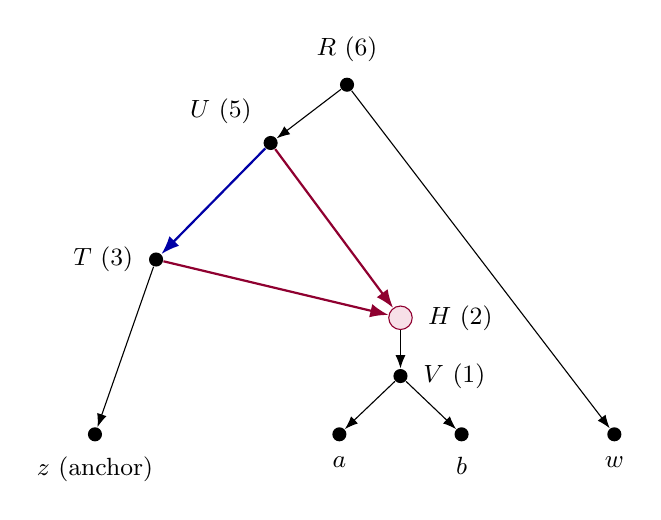
\begin{tikzpicture}[x=.97cm,y=.74cm,>=Latex,
 vertex/.style={circle,fill=black,inner sep=1.8pt},
 retic/.style={circle,draw=purple!75!black,fill=purple!12,inner sep=3pt},
 every node/.style={font=\small},label distance=2pt]
\node[vertex,label=above:{$R\ (6)$}] (R) at (1.3,6) {};
\node[vertex,label=above left:{$U\ (5)$}] (U) at (.3,5) {};
\node[vertex,label=left:{$T\ (3)$}] (T) at (-1.2,3) {};
\node[retic,label=right:{$H\ (2)$}] (H) at (2,2) {};
\node[vertex,label=right:{$V\ (1)$}] (V) at (2,1) {};
\node[label=below:$a$,vertex] (a) at (1.2,0) {};
\node[label=below:$b$,vertex] (b) at (2.8,0) {};
\node[label=below:{$z$ (anchor)},vertex] (z) at (-2,0) {};
\node[label=below:$w$,vertex] (w) at (4.8,0) {};
\draw[->] (R)--(U); \draw[->] (R)--(w);
\draw[->,thick,blue!65!black] (U)--(T);
\draw[->,thick,purple!75!black] (U)--(H);
\draw[->,thick,purple!75!black] (T)--(H);
\draw[->] (T)--(z); \draw[->] (H)--(V);
\draw[->] (V)--(a); \draw[->] (V)--(b);
\end{tikzpicture}
\end{minipage}\hfill
\begin{minipage}[c]{.42\linewidth}
\centering\small
\textbf{Population parameters}\par\medskip
\begin{tabular}{@{}lcc@{}}
\toprule
Arc & Rate & Weight at $H$ \\
\midrule
$T\to H$ & $\lambda_1=1$ & $\gamma=1/3$ \\
$U\to H$ & $\lambda_2=2$ & $1-\gamma=2/3$ \\
$U\to T$ & $\lambda_o=3$ & --- \\
\bottomrule
\end{tabular}
\par\medskip
Weights specify the backward choice\par
from $H$ toward $T$ or $U$.
\par\medskip
Diagnostic triple: $(a,b,z)$.\par
The anchor is $z$; $w$ is not used.
\end{minipage}
\caption{Worked graph for \cref{ex:worked-inverse}. Arrows point from older
populations toward descendants; the NMSC runs upward. The two purple arcs
meet at the reticulation $H$, and the blue arc carries the known first-route
mass after the earlier parent. Arc parameters and backward routing weights
are listed separately at right. Ages are shown in parentheses; all leaves
have age zero and all unlisted rates are one.}
\label{fig:worked-inverse}
\end{figure}

\begin{corollary}[Recovered population ports and decorated words]
\label{thm:bridge}
\label{lem:canonical-port-gluing}
The law determines every exposed population incidence, bridge, blob, and
ordered demographic or side-port word of the normalized graph, modulo
Q1--Q8.  Their conditional NMSC responses and common-boundary compositions
are then determined by the recovered positive graph and parameters.
\end{corollary}
\begin{proof}
These are graph features or forward transition laws of the object recovered
in \cref{thm:structural-inverse,thm:numerical-inverse}.  Their labels,
times, and incidences are global vertex data; matching them requires no
independent minimal-realization basis or historical route projector.
\end{proof}

\begin{lemma}[Strong-fan stopping and anchor theorem]
\label{lem:strong-fan}
Every nontrivial maximal pre-exposure unary fan has one hidden reticulation
and two typed first-exposure outlets.  Its only retained stochastic datum
is the paired outlet weight $(\gamma,1-\gamma)$, modulo parent presentation.
Distinct maximal fan interiors are disjoint.
\end{lemma}
\begin{proof}
A reticulation with only one descendant sample is immediately above its
singly sampled terminal by \cref{lem:cluster-poset}.  Each parent is a
tree vertex whose other child is ordinary.  A tree-only witness from that
child reaches the parent deterministically, so that route's first possible
pair exposure is exactly the parent boundary.  The incoming edge has no
side entry, and the fan stops before it can encounter another reticulation.
The two parents have distinct times.  The earlier parent's witness
distinguishes its outlet over the positive interval before the other
parent, as in \cref{lem:oriented-inheritance}.  Conversely, any routed
pre-exposure unary fan has only one descendant label and so is of this
form.  If different focal-label fans shared an interior population, their
two labels could co-occupy it with positive probability, a contradiction.
For one focal label maximality combines overlapping initial unary regions.
\end{proof}

\begin{example}[Exact in-class reticulation-time slide]
\label{ex:unary-fan-slide}
Consider the binary raw network
\[
 R\to S,\ R\to w,\qquad
 S\to T,\ S\to X,\qquad
 T\to z,\ T\to X,\qquad X\to x,
\]
where $X$ is reticulate, $x,z,w$ are sampled leaves, and
\[
 0<h=\tau_X<a=\tau_T<d=\tau_S<r=\tau_R.
\]
The blob is the cycle $S$--$T$--$X$--$S$.  The two reticulation-arrow
tails $S,T$ have ordinary incidences $(R\!-
S,S\!-\!T)$ and $(S\!-\!T,T\!-\!z)$, so this is a strict level-one
minimum strong repair, not a boundary degeneration.

Let the sole child block $x$ choose the $T$ arm with probability
$\gamma\in(0,1)$.  Before time $a$ every routed lineage is alone.  If the pair
rate on $S$--$T$ is $\lambda>0$ and $\Delta=d-a$, then
\[
 f_{xz}(a+u)=\gamma\lambda e^{-\lambda u},\quad 0<u<\Delta,
 \qquad
 \Pr\{xz\text{ survives to }d\}=1-\gamma+\gamma e^{-\lambda\Delta}.
\]
Equivalently, the complete local unmerged/merged kernel is
\[
 K_{a,d}=
 \begin{pmatrix}
 1-\gamma+\gamma e^{-\lambda\Delta}&
 \gamma(1-e^{-\lambda\Delta})\\
 0&1
 \end{pmatrix}.
\]
It is independent of $h$ and of every rate on the singly occupied incident
arms.  The state at $d$ is also independent of $h$, so composing with the
lineage $w$ and any common upper context preserves equality.  Every
$h,h'\in(0,a)$ therefore gives the same complete metric-genealogy law.  The
fan has lower boundary $x$ and upper exits $T@a,S@d$ with transport weights
$\gamma,1-\gamma$.  It is not a sample-unary corridor because it has two upper
boundaries before exposure.  This example forces move (Q8).
\end{example}


\section{One-reticulation normal form and the triangle theorem}
\label{sec:triangle}

\begin{theorem}[One-reticulation classification]
\label{thm:one-retic}
A normalized strict one-reticulation presentation is determined by its
metric-genealogy law up to parent presentation, sample-unary contraction,
pre-exposure unary-fan replacement, and bi-unary sister-triangle reversal with
the entire exposed donor-rate-word transfer.  If the reticulation is pair exposed, its time, child
and parent incidences, physically linked exposed rates, and $\gamma$ modulo
parent exchange are pointwise identifiable.  If it is not exposed, only its
two typed fan outlets and paired route weights are retained.
\end{theorem}

\begin{proof}
Restrict the structural and numerical inverses
\cref{thm:structural-inverse,thm:numerical-inverse} to a single blob with one
reticulation.  They recover every retained incidence and exposed parameter.
The only incomplete graph completion is the bi-unary sister case, and the
only missing event time belongs to a singleton fan.  These have precisely
the Q6 and Q8 identities proved below.
\end{proof}

Let $a$ be the first time at which the routed block can co-occupy a donor
population with the opposite sister block, and let $d>a$ be their
reconvergence time.  Put $\Delta=d-a$.  Write $\lambda_D(a+u)$ for the positive finite
piecewise-constant exposed donor rate word on $0<u<\Delta$ and put
\[
 \Lambda_D(u)=\int_0^u\lambda_D(a+v)\,\dd v.
\]
Adjacent equal-rate pieces are already composed by Q3.  The internal
reticulation time $h<a$ is retained only when it is independently pair
exposed; otherwise it belongs to Q8.

\begin{lemma}[Bi-unary contextual kernel]
\label{lem:biunary}
With exactly one reachable block at each sister port, the local
unmerged/merged kernel from first exposure $a$ to reconvergence $d$, for
routing into a donor population with exposed rate word $\lambda_D(\cdot)$ and composite probability
$\gamma$, is
\[
 K(\gamma,\lambda_D(\cdot),\Delta)=
 \begin{pmatrix}
 1-\gamma+\gamma e^{-\Lambda_D(\Delta)}&\gamma(1-e^{-\Lambda_D(\Delta)})\\
 0&1
 \end{pmatrix},
\]
and the merger density at $a+u$ is
$\gamma\lambda_D(a+u)e^{-\Lambda_D(u)}$ away from its finitely many demographic
boundaries, with the corresponding one-sided densities at a boundary.  Reversal with the same joining probability,
the same typed exposure interval, and transfer of the entire exposed donor rate word, including every retained breakpoint, has
the same complete marked kernel in every common context.  The position and
factorization of any preceding unary fan are already quotiented by Q8.
\end{lemma}

\begin{proof}
With probability $1-\gamma$ the blocks remain in separate populations until $d$.  With probability $\gamma$ they share the donor population.  Conditional survival through $a+u$ is $e^{-\Lambda_D(u)}$, and the ordinary inhomogeneous Kingman hazard gives merger density $\lambda_D(a+u)e^{-\Lambda_D(u)}$ on each demographic chamber.  Cutting any complete ranked genealogy at the lower and upper boundaries factors its density into a lower scalar prefix, one entry of this local marked kernel, and an upper scalar continuation.  Equality of the whole transferred rate word therefore gives equality of all local entries and contextual equality.  The constant-rate formula is the one-piece special case, not an extra hypothesis of Q6.
\end{proof}

\begin{lemma}[Pair-exposed routing separation]
\label{lem:pair-exposed}
Let $x,y$ be distinct surviving blocks on one sister side.  In the direction
in which that side routes independently at time $h$, their conditional
no-merger survival immediately above $h$ is
\[
 2\gamma(1-\gamma)+\gamma^2e^{-\lambda_1u}
 +(1-\gamma)^2e^{-\lambda_2u}.
\]
In the reverse direction the pair does not route and its boundary-free
survival is one Kingman exponential $e^{-\lambda_0u}$.  These functions cannot
agree on a nonempty open interval for strict parameters.
\end{lemma}

\begin{proof}
The independent-routing expression has the strictly positive exponent-zero
atom $2\gamma(1-\gamma)$.  A positive finite exponential sum with that atom
cannot equal a positive-rate exponential on an open interval.  This remains
true when $\lambda_1=\lambda_2$, at $\gamma=1/2$, and when surrounding response
exponents repeat.
\end{proof}

\begin{proof}[Proof of \cref{thm:triangle}]
Bi-unary invisibility is the complete contextual kernel of
\cref{lem:biunary}, including its hidden-clock freedom.  Conversely the
structural inverse has only the two-singleton pendant triangle ambiguity.
If either side is pair exposed that exception is unavailable, so the common
signed pair supports force its direction.  The positive split component in
\cref{lem:pair-exposed} explains the local separation, including equal rates;
the signed-support argument justifies it from actual observed pair laws
without conditioning on a supplied hidden occupancy.
\end{proof}

\section{Level-2 cores and decorated reattachment}
\label{sec:cores}
After deleting pendant bridge components but retaining their attachment ports,
and suppressing unported ordinary degree-two vertices, a level-at-most-two blob
has one of five directed cores: one cycle and four theta orientations.  The
following result is proved directly from the graph axioms; no substitution
invariant, unpublished classification, or preloaded table is used as evidence.

\begin{proposition}[Five-core theorem]
\label{prop:five-core}
Every nontrivial suppressed binary rooted level-at-most-two blob is a directed cycle or one of four directed theta cores.  Every full strongly tree-child expansion is obtained by inserting ordered words of port-bearing tree vertices on directed core segments and contains one of twelve minimum strong repairs: two for the cycle, two each for theta cores $0,1,3$, and four for theta core $2$.
\end{proposition}

\begin{proof}
Let $G$ be the undirected multigraph obtained from one blob by retaining its
distinguished incoming boundary, forgetting ordinary directions, and
suppressing ordinary degree-two vertices without ports.  Biconnectedness
excludes a figure eight or two cycles joined by a bridge.  If the cyclomatic
number is one, $G$ is a cycle.  If it is two, then
\[
 \sum_{v\in V(G)}(\deg v-2)=2|E|-2|V|=2.
\]
The binary degree bound and minimum degree two imply exactly two degree-three
vertices; removing them leaves three internally disjoint paths between the
same endpoints.  Thus $G$ is a theta multigraph.  Enforcing acyclicity, one
incoming boundary, binary tree degrees, and exactly two indegree-two/outdegree-
one vertices yields four boundary-preserving directed theta orbits.  With the incoming source denoted $S$, their ordered arc lists are
\[
\begin{array}{c|l}
\text{cycle}& SX,SX\\
\theta_0& SU,SV,UX,VX,UV\\
\theta_1& SU,SX,VX,UV,UV\\
\theta_2& SU,SV,UX_0,VX_0,UX_1,VX_1\\
\theta_3& SU,SX_0,VX_0,UX_1,VX_1,UV.
\end{array}
\]
Arc indices below start at zero in this displayed order.  Repeated entries
are parallel suppressed segments, not parallel raw reticulation parents.  This is a finite
orientation check on the three path directions; reversing all directions is
excluded by the distinguished boundary, and every other assignment either has
a directed cycle, the wrong number of reticulations, or a nonbinary vertex.

For a fixed directed core, subdividing a segment by a port-bearing tree vertex
is a Boolean choice.  Exhaust all $2^m$ subsets ($m=2,5,5,6,6$), build the raw
multidigraph with compulsory path-sink children, and impose both the rooted
tree-child condition and the strong local-tail condition at every reticulation
arrow.  Removing every nonminimal satisfying subset leaves respectively
\[
 \{0\},\{1\};\quad
 \{2,3\},\{3,4\};\quad
 \{2,3\},\{2,4\};\quad
 \{2,3\},\{2,5\},\{3,4\},\{4,5\};\quad
 \{2\},\{4\}.
\]
The supplement gives the primitive degree predicates and the independent
enumeration algorithm.  Every larger strong expansion contains a minimal
satisfying subset, and its remaining vertices form ordered port words on core
segments.  This proves both exhaustion and the count twelve.
\end{proof}

\begin{theorem}[Decorated-core reattachment injectivity]
\label{thm:reattach}
For every cycle or theta core, every strong repair, and arbitrary finite
ordered side-port words and nested pendant components, the labelled retained
event clusters, times, signed pair supports, and numerical data of
\cref{thm:numerical-inverse} determine the original normalized local quotient.
\end{theorem}
\begin{proof}
Apply the global cluster-poset and shortcut-completion argument of
\cref{thm:structural-inverse} to all retained vertices.  Each additional
side-port vertex has its own observed tree event, labelled descendant cluster,
and temporal coordinate; each nested component contributes vertices in the
same global poset.  Every cover edge and every non-Q6 shortcut is therefore
fixed, irrespective of the number of decorations.  The rate words and
inheritance data on the fixed incidences are determined by
\cref{thm:numerical-inverse}.  Thus reattachment is injective directly on
arbitrary expansions.  The finite minimum-core enumeration is not a premise
for the arbitrary-word step.
\end{proof}

\begin{theorem}[Three-lineage labelled marginal reconstruction]
\label{cor:three-suffice}\label{thm:three}
Let $\mathcal A_3(\bar\mu)$ be the indexed family of all induced genealogy
laws on $T\subseteq S$ with $|T|\le3$. On the same fixed
$(X,S,\mathfrak s)$ and the full class of \cref{thm:main},
\[
 \mathcal A_3(\bar\mu)=\mathcal A_3(\bar\mu')
 \quad\Longleftrightarrow\quad
 \Qraw(N,\bar\eta;\mathfrak s)=\Qraw(N',\bar\eta';\mathfrak s).
\]
This is a sufficient bound for the complete indexed family; it asserts
neither recovery from one fixed triple nor minimality of three.
\end{theorem}
\begin{proof}
Every pair law is included, so \cref{thm:structural-inverse} determines one
common global labelled graph, with the same retained vertices, clusters,
chronology and incidences. Choose the same Q6 orientation and the same
 graph-selected witnesses in both realizations. Every formula in
\cref{thm:numerical-inverse} uses a pair or triple law and therefore recovers
identical parameters on those common incidences. The grouping mass $q_3$
uses no merger in its own selected triple, not survival of all labels in
$S$. Sampling consistency supplies these quantities from $\mathcal A_3$;
forward propagation on recovered parameters adds no observation. Thus no
union of all witness labels is needed in one marginal. Conversely each
quotient move preserves the full law and hence every selected marginal.
\end{proof}

\begin{corollary}[Eight-lineage consequence]
\label{thm:eight}
Let $\mathcal A_8(\bar\mu)$ be the indexed family of all induced genealogy
laws on $T\subseteq S$ with $|T|\le8$. On the same domain,
\[
 \mathcal A_8(\bar\mu)=\mathcal A_8(\bar\mu')
 \quad\Longleftrightarrow\quad
 \Qraw(N,\bar\eta;\mathfrak s)=\Qraw(N',\bar\eta';\mathfrak s).
\]
\end{corollary}
\begin{proof}
This family contains $\mathcal A_3$, so \cref{cor:three-suffice} gives the
forward implication. Quotient soundness gives the converse. The same
argument applies to every integer upper bound at least three.
\end{proof}

\section{Global raw-to-raw proof}
\label{sec:global}

\begin{proof}[Proof of \cref{thm:main}]
For the forward implication, equality of the complete laws gives equality
of their labelled pair laws by sampling consistency.  The frozen positive
germ yields the same unnormalized co-occupancy functions.  Their signed
jumps identify the same retained biological events and clusters, and
\cref{thm:structural-inverse} identifies the same global graph modulo the
declared Q6 orientation.  Contracted unary reticulations retain their two
parent incidences and have exactly the Q8 clock freedom.

Choose a common canonical Q6 orientation, using the contextual identity
\cref{lem:biunary}.  All ordinary words then agree by
\cref{lem:ordinary-words}; oriented inheritance weights, including Q8
outlet weights, agree by \cref{lem:oriented-inheritance}.  The triple
first-and-second-merger density recovers each incoming word up to its
earlier parent.  Continuing the isolated longer-arm mass by
\cref{lem:incoming-long} recovers every remaining incoming word, with
ancestors processed before lower sinks.  No parameters are inferred from a
restriction after their witness labels have been removed.  All recovery
uses the original common labelled law.

Every biological incidence is part of one common global poset, so adjacent
blobs and arbitrary port words already have matching endpoints.  There is
no further reattachment choice or cross-blob gauge.  Parameter-free
subdivisions, equal-rate subdivisions, parent presentation, and unary
corridors differ only by Q1--Q5 and Q7; bi-unary donor transfer is Q6; and
unary fan clocks and words differ only by Q8.  This proves equality of the
declared raw quotient.

For the reverse implication, suppression and coincident-boundary
composition preserve the transition law; equal-rate merging is semigroup
composition; singleton corridors have no Kingman event; parent exchange
renames Bernoulli outcomes; and labelled isomorphism preserves the entire
process.  The exact Q6 contextual kernel is \cref{lem:biunary}.  A Q8 fan
has no internal merger and transports its one block to the same two typed
outlets with the same weights, so it preserves every complete marked
genealogy probability in any common exterior context.  Thus all eight
generators preserve the full law, proving the converse.
\end{proof}

\section{Parameter and sampling fibers}
\label{sec:parameters}

\begin{theorem}[Population-rate criterion]
\label{thm:rates}
On the stated strict class, every pair-exposed population rate word is
pointwise identifiable on its recovered incidence, modulo the Q6 donor-word
transfer.  A population with at most one reachable sampled block has no
observable rate.  Adjacent equal-rate epochs on an unchanged exposed
population are one quotient epoch.
\end{theorem}
\begin{proof}
For ordinary arcs use the deterministic witness and $f/q$ formula;
for reticulation-parent arcs use
\cref{lem:incoming-first,lem:incoming-long}.  These exhaust the exposed
arcs and prove physical incidence linkage, even when rates coincide.
On an unexposed arc the Kingman factor is $\binom12=0$, so changing its
positive rate word affects no genealogy.  Q3 and Q6 have the stated exact
identities.
\end{proof}

\begin{theorem}[Reticulation-time criterion]
\label{thm:event-time}
A reticulation time is pointwise identifiable exactly when its child is pair
exposed.  Otherwise it is the unary clock inside Q8; the law retains its two
typed parent outlets and paired weights, and its time can vary within the
compatible strict positive interval.
\end{theorem}
\begin{proof}
Pair exposure gives the nonzero negative jump in
\cref{lem:signed-jumps}.  In its absence the reticulation is directly above
a singly sampled terminal and its two incoming arms have no possible
merger.  Moving it below the two fixed parent times preserves its fan
response, as in \cref{ex:unary-fan-slide}.
\end{proof}

\begin{theorem}[Inheritance and direction fibers]
\label{thm:inheritance}
Every retained inheritance probability is identified as the weight of its
typed parent outlet, modulo parent exchange and the bi-unary sister
equivalence.  Q8 removes its unary clock and unary demographic words, not
its weight.  Every nonsister direction is retained.  A sister direction is
retained exactly when at least one side is pair exposed.
\end{theorem}
\begin{proof}
The oriented jump formula is \cref{lem:oriented-inheritance}.  The only
graph completion ambiguity in \cref{thm:structural-inverse} is the pendant
two-terminal bi-unary triangle, whose complete numerical fiber is
\cref{lem:biunary}.  Thus no posterior-balanced switching of parent words
survives the recovered physical incidences.
\end{proof}

\begin{theorem}[Terminal population rate]
\label{thm:terminal}
The terminal population rate of taxon $x$ is identifiable if and only if $m_x=|\mathfrak s^{-1}(x)|\ge2$.
\end{theorem}

\begin{proof}
With two terminal blocks, their merger density and no-merger survival on the terminal interval identify the rate.  With one block no Kingman event can occur there, so the rate is absent from every genealogy law.
\end{proof}

\begin{remark}[Physical scale]
The companion study \citep{KriebelNMSCCore2026} identifies normalized times and rates.  For one fixed normalized physical realization, the remaining conversion to physical units is
\[
 (\tau,\lambda,Q)\mapsto(c\tau,\lambda/c,Q/c),\qquad c>0.
\]
Other graph and parameter moves in the raw quotient may enlarge the complete
observational fiber.  It is not scale-only.
\end{remark}

\section{Comparison with triangle-forgetting topology}
\label{sec:comparison}
Define a formal semi-directed triangle-forgetting quotient $\Qdirect$ by
forgetting the root and demographic coordinates and every ordinary
sister-triangle orientation, with the same labelled graph conventions as
above.  Define its fan-compatible version $\widetilde\Qdirect$ as follows: begin
with the canonical compound Q6--Q8 response macros, retain their typed incidences, and
forget the root, demographic coordinates, and every ordinary sister-triangle
orientation.  This definition is a graph forgetful operation.  It does not
assume a global sitewise-model classification from the direct-substitution
papers.

\begin{theorem}[Comparison theorem]
\label{thm:comparison}
There is a natural forgetful map
\[
 \Qraw(N,\eta;\mathfrak s)\longrightarrow\widetilde\Qdirect(N).
\]
It loses direction on pair-exposed sister triangles, whereas the NMSC law
retains that direction.  The bi-unary sister reversal is already quotiented
on the NMSC side.  No map from a hidden fan clock to a distinguished ordinary
raw graph is required.
On the fan-rigid subdomain, where every retained reticulation is pair exposed,
the map further reduces to $\Qdirect(N)$.  It is strict on pair-exposed sister
triangles.  For the local bi-unary sister module, both quotients identify
the two directions.
\end{theorem}
\begin{proof}
Q1--Q5 and Q7 preserve the stated normalized incidences, Q6 forgets a
sister orientation already absent in the target, and Q8 preserves its typed
macro by definition.  The map is therefore well defined.  When every
reticulation is exposed there are no Q8 macros, giving the further map.
The strictness and local direction equivalence follow from
\cref{thm:triangle,lem:biunary}.
\end{proof}

Direct-substitution model questions and this pointwise NMSC question use
different observations and quantifiers.  A global identification of the
formal target with a common JC/K2P/K3P statistical-model quotient additionally
requires the exact cross-paper translation of graph conventions and local
relations.  That translation is not a premise or a consequence of the
present NMSC proof.

\section{Finite locus consequence and reconstruction scope}
The companion study \citep{KriebelNMSCCore2026} proves that on every fixed finite union $K$ of compact semianalytic normalized finite-presentation charts there is a finite $L_*(K)$ such that equality of the length-$L_*(K)$ law is equivalent to equality of all indexed laws.  Combining that theorem with \cref{cor:sequence} gives finite determination of $(\pi,Q_0,\Qraw)$ on the corresponding compact semianalytic level-2 charts.  No effective practical sequence-length bound is claimed here.

The present graph reconstruction is exact from the metric-genealogy law or from all indexed sequence laws through the companion study.  It is not advertised as a polynomial-time inference method and supplies no finite-sample accuracy guarantee.  The exact software checks finite proof interfaces and hostile boundary examples; it is supplementary evidence, not a substitute for the universal proof.

\section{Scope, novelty, and nonclaims}
The graph inverse uses no Fourier coordinate, group-based invariant, or
site-pattern rank.  It makes no appeal to triangle varieties from direct
substitution models.  It depends only on the normalized genealogy law and is
therefore uniform within the companion study's stated reversible substitution class.
The cycle/theta core list and its twelve minimum repairs are independent
graph results.  Decorated reconstruction uses the global signed-jump
cluster poset for every finite expansion.

The full-likelihood literature documents bidirectional-introgression label
switching and the ability of multiple sampling to help identify sister
introgression direction \citep{YangFlouri2022,ThawornwattanaEtAl2023}.
Simultaneous-BDI switches are not imported into this temporally separated
quotient.  The result here is the pointwise graph-and-parameter
classification, including the exact exposure criterion, typed unary-fan
fiber, whole demographic words, and the stated finite labelled-marginal
bound.

No claim is made for level three, unknown nonreversible generators, unknown
locus boundaries, within-locus recombination, arbitrary rate mixtures,
practical finite-sample reconstruction, or empirical adequacy.

\section{Proof audit summary}
The analytic inverse is supplied in the main text and expanded in the
technical supplement.  Its ingredients are sampling consistency, current
positive-mixture grouping germs, signed pair supports, tree-child ancestry
from clusters, level-two shortcut completion, and explicit numerical
formulas on the recovered graph.  Historical-signature projectors and
arbitrary-candidate fan-code predicates are not proof inputs.

Exact computations check the primitive core and minimum-repair lists,
minimum-row signed-support signatures, and all single-side-port insertions
under the declared finite enumerations.  These checks support the proofs at
those exact scopes; they do not certify arbitrary expansions by themselves.
The structural proof treats those expansions directly.  Executed software
coverage and reproduction instructions are reported separately in the
submission certificate.

\begin{thebibliography}{99}
\bibitem[Hellmuth et al.(2023)]{HellmuthSchallerStadler2023}
M. Hellmuth, D. Schaller, and P. F. Stadler. Clustering systems of phylogenetic networks.
\emph{Theory in Biosciences}, 142:301--358, 2023. doi:10.1007/s12064-023-00398-w.
\bibitem[Kriebel(2026)]{KriebelNMSCCore2026}
A. Kriebel. \emph{Direct Sequence Laws under the Network Multispecies Coalescent: A genealogy equivalence, canonical coalescent-response behavior, and finite determination with an epoch-complexity obstruction}. Preprint, Zenodo, 2026. \href{https://doi.org/10.5281/zenodo.22729537}{doi:10.5281/zenodo.22729537}.
\bibitem[Yang and Flouri(2022)]{YangFlouri2022}
Z. Yang and T. Flouri. Estimation of cross-species introgression rates using genomic data despite model unidentifiability. \emph{Molecular Biology and Evolution}, 39(5):msac083, 2022. doi:10.1093/molbev/msac083.
\bibitem[Thawornwattana et al.(2023)]{ThawornwattanaEtAl2023}
Y. Thawornwattana, J. Huang, T. Flouri, J. Mallet, and Z. Yang. Inferring the direction of introgression using genomic sequence data. \emph{Molecular Biology and Evolution}, 40(8):msad178, 2023. doi:10.1093/molbev/msad178.
\bibitem[Allman et al.(2024)]{AllmanBanosGarroteRhodes2024}
E. S. Allman, H. Ba\~nos, M. Garrote-L\'opez, and J. A. Rhodes. Identifiability of level-1 species networks from gene tree quartets. \emph{Bulletin of Mathematical Biology}, 86:110, 2024. doi:10.1007/s11538-024-01339-4.
\bibitem[Allman et al.(2023)]{AllmanBanosMitchellRhodes2023}
E. S. Allman, H. Ba\~nos, J. D. Mitchell, and J. A. Rhodes. The tree of blobs of a species network: identifiability under the coalescent. \emph{Journal of Mathematical Biology}, 86(1):10, 2023. doi:10.1007/s00285-022-01838-9.
\bibitem[Zhu and Degnan(2017)]{ZhuDegnan2017}
S. Zhu and J. H. Degnan. Displayed trees do not determine distinguishability under the network multispecies coalescent. \emph{Systematic Biology}, 66(2):283--298, 2017. doi:10.1093/sysbio/syw097.
\bibitem[Allman et al.(2025)]{AllmanAneBanosRhodes2025}
E. S. Allman, C. An\'e, H. Ba\~nos, and J. A. Rhodes. Beyond level-1: identifiability of a class of galled tree-child networks. \emph{Bulletin of Mathematical Biology}, 2025. doi:10.1007/s11538-025-01545-8.
\bibitem[Holtgrefe et al.(2025)]{HoltgrefeEtAl2025}
N. Holtgrefe, E. S. Allman, H. Ba\~nos, L. van Iersel, V. Moulton, J. A. Rhodes, and K. Wicke. Distinguishing phylogenetic level-2 networks with quartets and inter-taxon quartet distances. \emph{Bulletin of Mathematical Biology}, 87:168, 2025. doi:10.1007/s11538-025-01549-4.
\bibitem[Holtgrefe et al.(2026)]{HoltgrefeEtAl2026Correction}
N. Holtgrefe, E. S. Allman, H. Ba\~nos, L. van Iersel, V. Moulton, J. A. Rhodes, and K. Wicke. Correction: Distinguishing phylogenetic level-2 networks with quartets and inter-taxon quartet distances. \emph{Bulletin of Mathematical Biology}, 2026. doi:10.1007/s11538-025-01564-5.
\end{thebibliography}
\end{document}
